\chapter{Continuing Work}
\label{sec:continue}

(Introduction part:
- commissioning will continue for all of this year
- moving from simulated studies to studies using data

Introduce the ways that your work is useful to commissioning:)

Input misalignments are a good way to retrieve information about how expected movements of the SciFi affect the alignment and monitoring outputs. When the data taking starts and and afterwards during times when the LHC is actively running, these simulated misalignment studies can be used for comparisons.
One sign of a good alignment is the absence of the layer splitting.
Similarly if the alignment is ``good'', in simulation it would converge towards the true aligned detector within three to five iterations.
If the convergence happens later there is either a bias hindering the alignment or there is a problem with the configuration itself.

After the work in this thesis there are still more open questions for the SciFi alignment. The cluster bias which prevents the alignment from working correctly is currently being analysed, and when this is fixed the alignment will require more testing with simulation and data.

Additionally, there is another weak mode to consider in the SciFi, called the curvature bias.
\begin{figure}
    \centering
    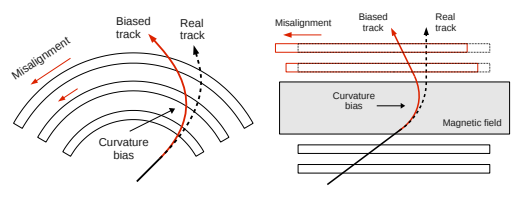
\includegraphics[width=0.8\textwidth]{plots/curvature_bias.png}
    \caption{Illustration of a curvature bias in a central detector (left) and a forward detector (right).}
    \label{fig:curvature}
\end{figure}
The curvature bias can appear in forward spectrometers with dipole magnets like the LHCb experiment and cylindrical detectors with solenoidal magnetic fields as shown in figure \ref{fig:curvature}.
In forward spectrometers like LHCb, the curvature bias can be caused by a superposition of relative shearing and rotation of the detectors surrounding the magnet. If a curvature bias is present, the reconstructed invariant mass of a two-body decay will be shifted proportionally to the momentum difference of the daughter particles in the final state\cite{1207.4756}.
There are two different ways to control the curvature bias. That is why alignment with particles will have an important role.
Another way to constrain the curvature bias is to use magnet-off data, but this only works if the detectors do not move when the magnetic field is turned on. Recent commissioning measurements of LHCb show that the SciFi detector does move when the magnet turns on.
% how much more detail is needed? citing a paper describing one method is enough?

In order to perform a successful alignment for the SciFi Tracker the detectors upstream of the SciFi need to be installed and aligned as well.
An essential part of the alignment is using correctly reconstructed long tracks, therefore the VELO has to be aligned to reconstruct good long tracks for the SciFi.

% only some corrections left. also home stretch !
